\documentclass[12pt]{article} 

%\documentclass[11pt, onecolumn]{ieeeconf}
%\linespread{1.3}

\usepackage{graphicx}
\usepackage{graphics} % for pdf, bitmapped graphics files
\usepackage{epsfig} % for postscript graphics files
%\usepackage{mathptmx} % assumes new font selection scheme installed
\usepackage{times} % assumes new font selection scheme installed
\usepackage{amsmath} % assumes amsmath package installed
\usepackage{amssymb}  % assumes amsmath package installed
\usepackage{bm}  % assumes amsmath package installed
\usepackage{enumerate}  % assumes amsmath package installed
\usepackage{hyperref}
\usepackage{color}

\def\bs{\boldsymbol}
\def\mb{\mathbb}
\def\cw{3.45in}
\def\ts{\textsuperscript}
\newcommand{\norm}[1]{\lVert#1\rVert}

\title{Peregrine: help}

%%% first author
\author{Sachit Butail}

\date{}


\begin{document}

\maketitle
\thispagestyle{empty}
\pagestyle{empty}

%%%%%%%%%%%%%%%%%%%%%%%%%%%%%%%%%%%%%%%%%%%%%%%%%%%%%%%%%%%%%%%%%%%%%%
%\begin{abstract}
%Peregrine is an automated tracking system for studying collective animal behavior. 
%\end{abstract}


%%%%%%%%%%%%%%%%%%%%%%%%%%%%%%%%%%%%%%%%%%%%%%%%%%%%%%%%%%%%%%%%%%%%%%
\section{Introduction}
\begin{figure}[ht]
\centering
\includegraphics[width=.995\linewidth]{screenshot}
\caption{Tracking shape and orientation of three fish in a flow tank.}
\label{fig:sample_tracks}
\end{figure}

\begin{figure}[ht]
\centering
\includegraphics[width=.995\linewidth]{output}
\caption{Output of the tracker is stored in a csv file where each \textbf{row} corresponds to a single target in a single frame. Table \ref{tab:csvcolumns} lists the column ids. }
\label{fig:output}
\end{figure}
Peregrine is an automated tracking system developed to analyse and study animal behaviour. Versions of this tracking system have been used/developed as part of \cite{Butail2011,Butail2012b,Butail2012c, Butail2013c, Ladu2014, Bartolini2014}. Please refer to those for technical details. This document describes basic steps to get started and use peregrine. 

\section{Initial setup}
\begin{figure}[ht]
\centering
\includegraphics[width=.295\linewidth]{prefs}
\caption{Preferences}
\label{fig:prefs}
\end{figure}

\begin{figure}[ht]
\centering
\includegraphics[width=.995\linewidth]{thresholds}
\caption{Setting thresholds to achieve the best possible tracking performance. (a) raw video; (b) with background checked and thresholds set; and (c) after selecting ``mark'' in the view type. Note the circular region of interest (ROI) as a blue dotted line.}
\label{fig:thresholds}
\end{figure}
Peregrine is developed in MATLAB and shared using a dropbox folder. For best results the input to peregrine should be in the form of frames with sequential filenames. The length of each filename should be the same, for example, exp01\_001.bmp, exp01\_002.bmp, exp01\_003.bmp, and so on. 
\begin{enumerate}
\item Ensure all video frames are in a single folder
\item Change MATLAB current folder to where peregrine is located
\item Type \emph{peregrine} on the command window and select File $\rightarrow$ open. Select any frame from the list of frames.
\item Press start to check if the video is playing properly.
\item Check the Background checkbox. Now, using the sliders ``Target contrast'' and ``Target intensity'' try to have the foreground only visible as white blobs on the screen. \textcolor{blue}{Set ``Target contrast'' to 0 if the targets are moving very slowly or remain still in some frames.}
\item Use the crop tool next to the background to Crop a region of interest; you may also remove unwanted areas within the region of interest using the button next to it (not recommended as this will also make the targets invisible if they enter such region, however recommended if there is a persistent noise source in that area).
\item Select the ``Mark'' radio button in the View type to see if all targets are selected (Fig. \ref{fig:thresholds}). Verify the count status on the right of the ``Live'' button.
\item Select Edit $\rightarrow$ preferences to set preferences (Fig. \ref{fig:prefs}). Most values can remain as default except ``Region of Interest (ROI) size (length, breadth in cm)'' and ``Shape of ROI (0=square, 1=circle)'', which should be specified as per the video. Setting ``Split occlusions=1'' allows occlusions to be resolved but should only be used if the target shapes can be approximated as ellipses (e.g. fish, bugs)
\item If you obtain consistent targets and most of your targets are seen marked in the ``mark'' view-type, then press save and move to Tracking.
\end{enumerate}


\section{Tracking}
Peregrine allows two types of tracking: position and shape. Position tracking outputs the target position and velocity for multiple targets and shape tracking outputs shape information in the form of coefficients of a parabola fit on the target midline. 
\subsection{Position and velocity tracking}
Position and velocity tracking uses a Kalman filter \cite{BarShalom1987}, and global data-association \cite{Kuhn1955} to track multiple targets in a video. To start tracking, first check that all preferences are set properly including \textcolor{blue}{ROI size and shape} and most targets are marked in most of the frames. Ensuring this will reduce the time spent in repairing the tracks. 

Now bring the slider to zero position and view-type to track. If you want to run the tracker without recording to see how the tracker performs press start. If everything looks okay, then stop, bring the slider back again and check the checkbox next to the track view to record the tracks. Now press start again. To speed up the tracker, you can toggle the ``live'' button. \textbf{Make sure to press save once the tracking is done}.
\subsection{Shape tracking}
The shape tracking follows the approach described in \cite{Bartolini2014}. Briefly, the measurements consist of a centroid, orientation, and two shape parameters that represent a parabola in the body frame. The parabola and corresponding orientation is found by brute-force search. The final measurements are fed into a particle filter with 200 particles. 
In the case of Shape tracking the csv file is ordered as:
\begin{table}[t]
\caption{csv file output for  tracking}
\begin{center}
%\rowcolors{1}{}{lightgray}
%\resizebox{\textwidth}{!}
\end{center}
\label{tab:csvcolumns}
\end{table}


\subsection{Repair mode}
The repair mode allows the user to fix the tracks by
\begin{enumerate}
\item Stitch broken tracks
\item Switch tracks before and after an occlusion that was not resolved properly
\item Add a new point for an undetected target
\end{enumerate}

\subsection{Command line mode}
\emph{pg\_cmd}
\section{Global observations}

Once trajectory data is available, the command \emph{get\_obs} computes the  various measures of collective behavior. We assume that both position and velocity of each target (for example fish) is available at all times during the experiment. We also assume that the each fish identified by a unique number that can be used to quantify the behavior during the trial. Unless specified, we make the assumption that the heading is the same as the direction of motion. (This assumption is dropped, for example, when the fish are in a water tunnel.)

\begin{enumerate}
\item \emph{Group cohesion:} The degree of cohesion in groups is described in terms of the average nearest-neighbor distance (ANND) \cite{Webster2007, Kolpas2008}. Given the two-dimensional position $\bs{r}_i[k]$ of the $i$-th fish at frame $k$, the ANND during that frame is \cite{Kolpas2008}
\begin{equation}
\mathrm{ANND}[k]=\frac{1}{N}\sum_{i=1}^N\min_{j\in \{1,\ldots,N\}, j\ne i}(\norm{\bs{r}_i[k]-\bs{r}_j[k]}),
\end{equation}
where $N$ is the total number of fish and $\norm{\cdot}$ denotes the standard Euclidean norm. 
\item \emph{Group coordination:} is captured through the polarization (Pol) that measures the degree of alignment between the directions of motion of the fish \cite{Vicsek1995}. Given the two-dimensional velocity $\bs{v}_i[k]$ of the $i$-th fish at frame $k$, the polarization at that frame is
\begin{equation}
\mathrm{Pol}[k]=\frac{1}{N}\Big\|\sum_{i=1}^N\hat{\bs{v}}_i[k]\Big\|, 
\end{equation} 
where $\hat{\bs{v}}_i[k] =\frac{\bs{v}_i[k]}{\norm{\bs{v}_i[k]}}$ is the direction of motion. 
\item \emph{Group speed:} is computed to describe average speed of the subjects, and is  given by 
\begin{equation}
S[k]=\frac{1}{N}\sum_{i=1}^N\|\bs{v}_i[k]\|
\end{equation}
\item \emph{Group angular momentum}: the normalized group angular momentum $\hat{L}$ is indicative of milling patterns \cite{Chuang2007, Couzin2003a}, with $\hat{L}=1$ for single milling formations and  $\hat{L}=0$ for a coherent one-directional formation \cite{Chuang2007}. Depending on how $\bs{r}_i$ is defined, the angular momentum can be computed about the group center of mass \cite{Aureli2012}, or about the center of the observation region.
\begin{equation}
\hat{L}[k]=\frac{\|\sum_{i=1}^N\bs{r}_i[k]\times\bs{v}_i[k]\|}{\sum_{i=1}^N\|\bs{r}_i[k]\|\|\bs{v}_i[k]\|}
\end{equation}
\item \emph{Group interaction:} with a focal fish (or an external stimulus such as a robot) is quantified in terms of values such as distance, alignment and relative speed. We denote the focal fish or target index with a subscript $\bs{r}_f$. Specifically the observables are
	\begin{enumerate}
		\item \emph{Average distance to the focal fish:} Average distance of all other fish to the focal fish
		\begin{equation}
			\hat{d}[k]=\frac{1}{N-1}\sum_{i\in\{1,\ldots,N\}, i\ne f}\|\bs{r}_i[k]-\bs{r}_f[k]\|
		\end{equation}
		\item \emph{Minimum distance to the focal fish:} Minimum distance to the focal fish between all other fish
		\begin{equation}
		\tilde{d}[k]=\underset{i\in\{1,\ldots,N\}, i\ne f}{\operatorname{argmin}}\|\bs{r}_i[k]-\bs{r}_f[k]\|
		\end{equation}
		\item \emph{Group relative speed with respect to the focal fish:}
		\begin{equation}
		\tilde{S}[k]=\Big(\frac{1}{N-1}\sum_{i\in\{1,\ldots,N\}, i\ne f}\|\bs{v}_i[k]\|\Big)-\|\bs{v}_f[k]\|
		\end{equation}
		\item \emph{Alignment to the focal fish:}
	\end{enumerate}
\item \emph{Group behavior:} quantifies on an average the behavior of subjects such as percentage time spent freezing, thrashing, or swimming. These values allow us to determine if the subjects were in general scared or not. The specific observables are:
	\begin{enumerate}
		\item \emph{Time spent freezing:} To elucidate the behavior of the subjects, we score the time spent freezing during each trial. This value is computed automatically based on the condition that a fish is considered freezing during a frame if it spends two continuous seconds within a ball of radius of 2 cm \cite{Kopman2013}. Freezing is recorded if at least one fish satisfied this condition.
		\item \emph{Excursions of focal from shoal:} To measure the number of excursions from the shoal of a particular fish, we use the definition of shoal membership as described in \cite{Miller2011a}. In particular, we (i) compute the time series of average nearest neighbor distance of the focal fish,(ii) distribution of ANND for all fish over all frames is computed. Use the mode of this distribution as the threshold, divide the time series into segments where the individual's ANND goes above the mode, and (iii) find the distribution of the maximum ANND of each segment. The upper p=0.05 quantile of the max ANND distribution determines if a segment is an excursion or not. 
	\end{enumerate}
\item \emph{Tail-beat frequency:} Tail-beat frequency is computed using the tail-tip position estimated from the body frame location. For a signal $x$, the \emph{fft} routine implements the following DFT
\begin{equation}
X(k)=\sum_{j=0}^{N-1}x(j)\omega^{jk},
\end{equation}
where $\omega=\exp(-2\pi i /N)$ and $k \in \mathbb{Z}$, and $x(j)$ is the coefficient for the sinusoidal frequency $\omega^{jk}$, which is equal to $jk/N$. Since matlab returns a double sided spectrum of magnitudes, the amplitude is obtained by doubling the magnitude of $X(k)$. 
Also refer to the example in \url{http://www.mathworks.in/help/matlab/ref/fft.html}.  
\begin{figure}
\centering
\includegraphics[width=.995\linewidth]{tbf_computation}
\caption{Tail-beat frequency computation: (a) tail end of the fish in successive frames (increasing in time as the color changes from grey to dark, with 0 marking the fish body center) when the fish was not occluded and away from the tank wall; (b) detrended relative tail-tip position during that sequence; and (c) Fast Fourier transform of the tail-tip position for analysis in the frequency domain. The frequency with the maximum magnitude (here 4.2 Hz) is selected as the tail-beat frequency}
\label{fig:tbf_computation}
\end{figure}	

\begin{figure}
\centering
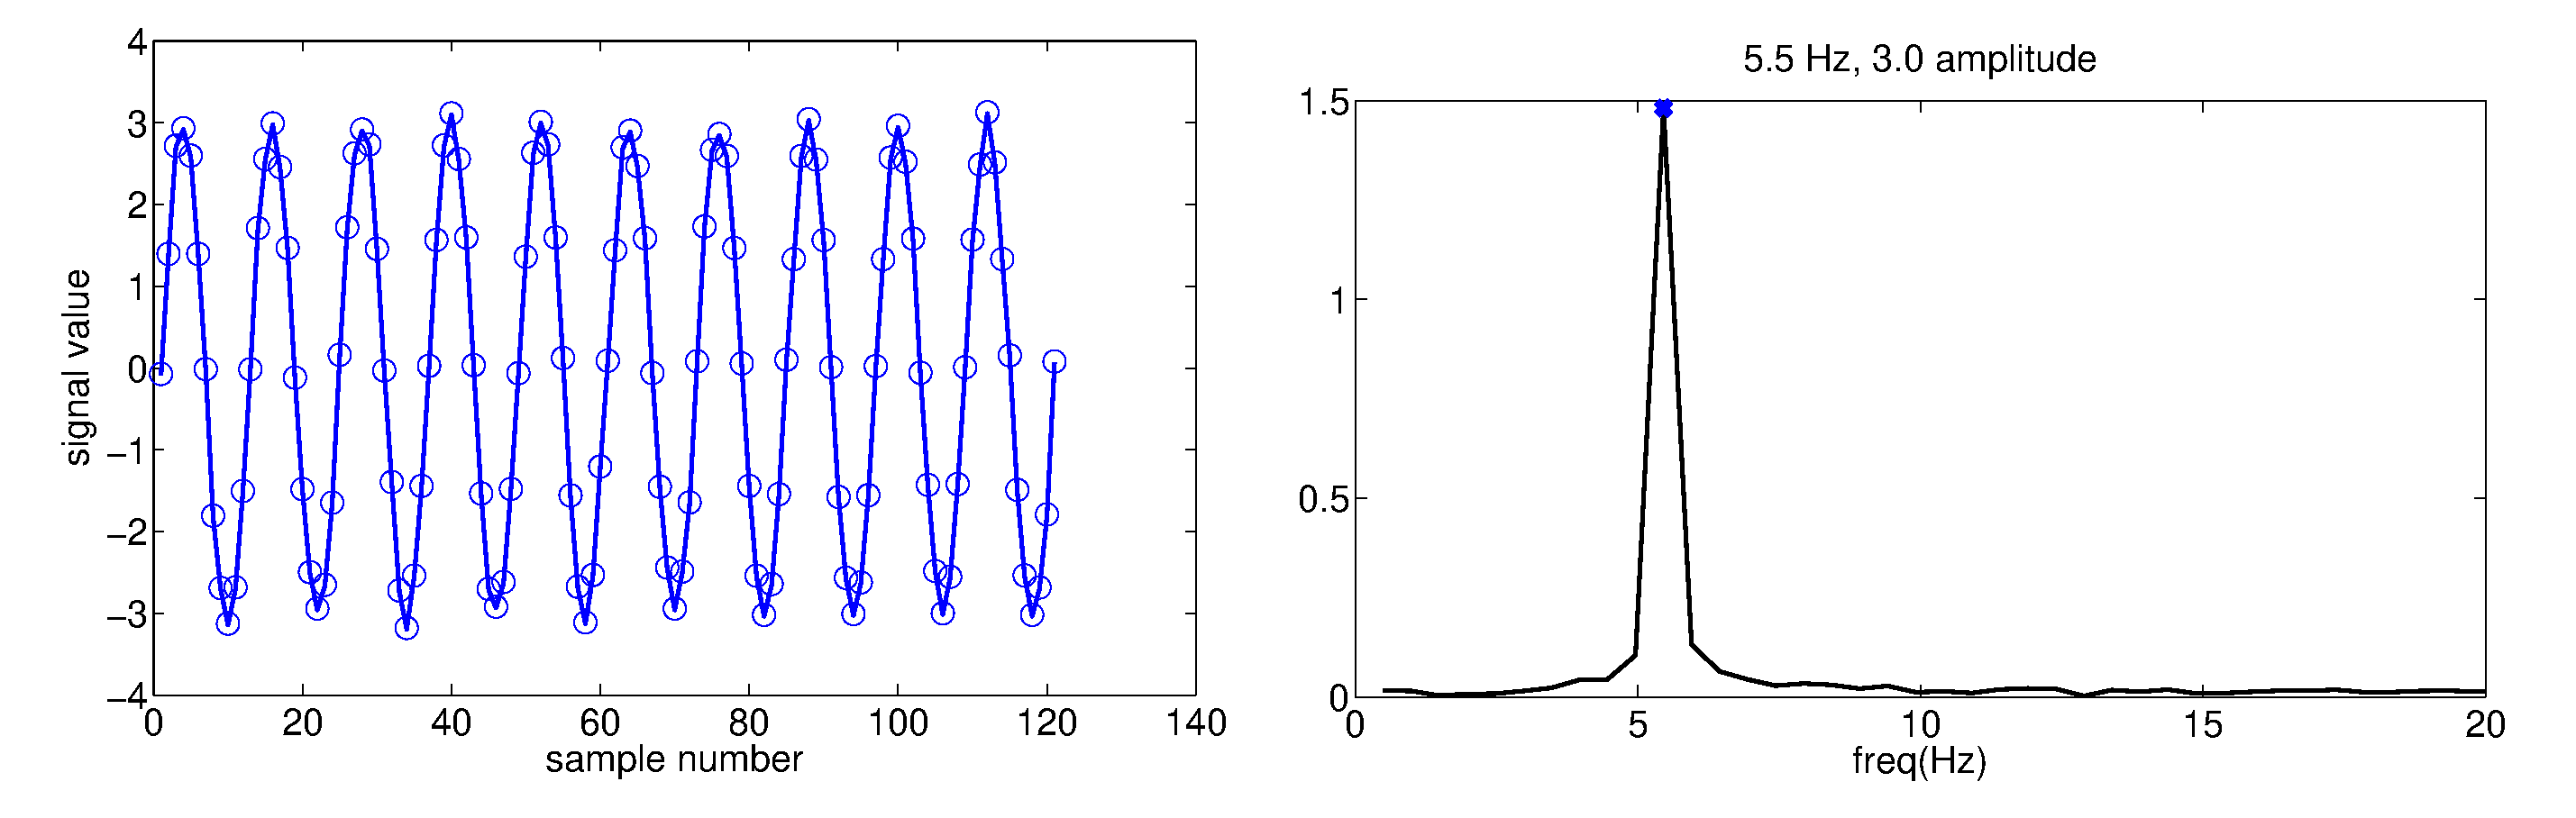
\includegraphics[width=.995\linewidth]{fft_example}
\caption{The toy example above shows how FFT is used to compute frequency and amplitude from a given signal. A signal with known frequency (5 Hz) and and amplitude (3 units) is sampled at 60 Hz after corrupting with zero-mean Gaussian noise of 0.1 units standard deviation. The signal is then detrended to remove linear trends. The circles on the left mark the detrended points on the noisy signal. The right plot shows the magnitude after applying the fast fourier transform along the length of the signal. The signal frequency is selected as the one where the magnitude is maximum (5.5 Hz) and the amplitude is twice the magnitude.}
\label{fig:fft_example}
\end{figure}	


\end{enumerate}


%%%%%%%%%%%%%%%%%%%%%%%%%%%%%%%%%%%%%%%%%%%%%%%%%%%%%%%%%%%%%%%%%%%%%%
\section{Acknowledgement}
The authors would like to acknowledge assistance (development and testing) from Dynamical Systems Laboratory, New York University, and Collective Dynamics and Control Laboratory, University of Maryland.

\bibliographystyle{unsrt}
\bibliography{$HOME/Reference/bibfiles/library}
\end{document}
